\chapter{Classification schemes}
In this chapter a few classification models are evaluated for the feature extraction processes described in the preceding chapter. Detailed descriptions of each classification framework is omitted, but good sources for further explanation will be supplied for the interested reader. The aim of this chapter is to compare various models and to determine the most promising one with regards to accuracy, size and complexity. 

The workflow for all models apart from the last one, follows the chart in figure \ref{fig:flow}, where both training- and test data is preprocessed before going into the classifier. 





% Define block styles
\tikzstyle{decision} = [diamond, draw, fill=blue!20, 
    text width=7.5em, text badly centered, inner sep=0pt]
\tikzstyle{block} = [rectangle, draw, fill=blue!20, 
    text width=7em, text centered, rounded corners, minimum height=4em]
\tikzstyle{line} = [draw, -latex']
\tikzstyle{cloud} = [draw, ellipse,fill=red!20, node distance=3cm,
    minimum height=4em]
\tikzstyle{blockgreen} = [rectangle, draw, fill=green!20, 
    text width=7em, text centered, rounded corners, minimum height=4em]
\tikzstyle{blockbrown} = [rectangle, draw, fill=brown!20, 
    text width=7em, text centered, rounded corners, minimum height=4em]

\begin{figure}
\centering
\begin{tikzpicture}[node distance = 3cm, auto]
	% Place nodes
	\node [blockbrown] (obtained) {Obtained data};
	\node [blockgreen, below left of=obtained] (training) {Training data};
	\node [block, below right of=obtained] (test) {Test data};
	\node [blockgreen, below of=training, node distance=2.2cm] (train pre) {Preprocess and extract features};
	\node [block, below of=test, node distance=2.2cm] (test pre) {Preprocess and extract features};
	\node [blockgreen, below right of=train pre] (est) {Estimate $\mathbf{\mu}_f$, $\mathbf{\sigma}_f$};
	\node [blockgreen, below left of=est] (scale train) {Scale to ZMUV};
	\node [block, below right of=est] (scale test) {Scale to ZMUV};
	\node [cloud, below right of=scale train] (train model) {Train model};
	\node [decision, below of=train model] (classify) {Classification};
	\node [block, below of=classify] (post) {Postprocessing};
	\node [block, below of=post, node distance=2.2cm] (output) {Model output};
	% Draw lines
	\path [line] (obtained) -| (training);
	\path [line] (obtained) -| (test);
	\path [line] (training) -- (train pre);
	\path [line] (test) -- (test pre);
	\path [line, dashed] (train pre) -| (est);
	\path [line,dashed] (est) -- (scale train);
	\path [line,dashed] (est) -- (scale test);
	\path [line] (test pre) -- (scale test);
	\path [line] (train pre) -- (scale train);
	\path [line] (scale train) |- (train model);
	\path [line] (train model) -- (classify);
	\path [line] (scale test) |- (classify);
	\path [line] (classify) -- (post);
	\path [line] (post) -- (output);
\end{tikzpicture}
\caption{Flowchart of classification scheme. Both training- and test data is preprocessed and scaled so that each feature has zero mean, unit variance. The training data is used to obtain model weighths, which become inputs to the classifier. Using these weights, predictions are made on the test data. These predictions then go through a postprocessing which results in the final output.}
\label{fig:flow}
\end{figure}






\section{Linear Models}
Linear models are widely used in practice as they are general, and can therefore be used in many cases \citep{shalev-shwartz_ben-david_2016}.  Furthermore, they are relatively easy to understand, in contrast to more complex models such as neural networks. Despite this, they can often produce a decent accuracy with a low complexity.

In this work, two linear models are considered. One being \emph{Linear Discriminant Analysis} (LDA) and the other, \emph{Support Vector Machine} (SVM) with a linear kernel. 

\subsection*{Linear Discriminant Analysis}
Linear Discriminant Analysis, or LDA for short, is an algorithm commonly used for dimensionality reduction of data. \citep{raschka_2014} It is not uncommon, however, to use it for classification tasks as well. LDA is a supervised algorithm, meaning it knows what class each sample belongs to. This enables it to project data into a lower dimension in such a way that the different classes are as separated as possible; unlike PCA which projects data in a way that maintains a high variance, disregarding class labels. 

Reducing the dimensionality of data is a good way of both lowering computational costs and avoiding overfitting as well as other phenomena that stem from a high-dimensional data. For further reading about LDA, we refer to \citep{raschka_2014}.

\subsection*{Support Vector Machine}
SVMs are one of the most popular models when it comes to supervised learning. The most simple SVM uses what is called a linear kernel, and generates a linear hyperplane that separates two sets of labeled data. Finding such a hyperplane is often an ambiguous task, so to find what the SVM regards as the best hyperplane, it seeks parameters that maximize the distance between the hyperplane and the sample points closest to it, known as support vectors \citep{boswell2002introduction}.

Even if support vector machines are linear models, they are not limited to work only on linearly separable data. There are ways to use them in a non-linear fashion by utilizing different kinds of kernels \citep{xia_2016}. In principle, the data is first transformed into a higher dimensional space, including non-linear terms. In this new space, the SVM is used just as before. This makes the SVM a powerful tool even in non-linear problems.

\section{Non-linear Models}
In some cases, the data is not linearly separable. That is, two classes in the dataset cannot be separated by any hyperplane. Hence, if a linear model were to be trained on data that is not linearly separable, one would expect to notice a poor result in comparison to the result of a non-linear model. 

The non-linear models considered in this work are random forest, logistic regression, as well as two kinds of neural networks.

\subsection*{Random Forest}
Random Forest (RF) is a strong tool that can be used for both regression- and classification problems. The name stems from that the method is based on several \textit{decision trees}, which are initiated randomly. A decision tree is a classifier per se, and is structured as a sequence of simple questions. These questions typically ask if a sample's feature is equal to, or greater/smaller than some set value. The answers to these questions form a path in the decision tree, leading to an end node which corresponds to the prediction.

RF segments the training data into $n$ parts, and induces a decision tree from each group of data. Thus there are $n$ predictors that work independently, and by selecting the most common prediction, RF yields a robust result with no overfitting due to the combined results of many trees. On top of that it offers a very high accuracy in a wide variety of applications, while still maintaining an intuitive model structure that allows us to, for instance, estimate which features are important. \citep{breiman_cutler_2018}


\subsection*{Logistic Regression}
Logistic regression is simlar to an ordinary linear regression. Both methods aim to estimate parameters to describe the relationship between the input- and the output variables. For linear regression, the parameters $\{b_i\}_{i=0}^n$ are estimated, and together with the input variables $\{X_i\}_{i=1}^n$ they generate the output $Y$:

\begin{equation}
	Y= b_0+\sum_{i=1}^n b_iX_i.
\end{equation}

One big difference between the two models is that linear regression outputs continuous values in $\mathbb{R}$, whereas logistic regression outputs a value in the open interval (0,1).  To achieve this, logistic regression transforms the result of the linear regression using the sigmoid function, defined as $f(z)=\frac{1}{1+e^{-z}}$. With this function, logistic regressions maps the inputs $X_i, i=1,...,n$ to
\begin{equation}
	Y= \frac{1}{1+e^{-b_0-\sum_{i=1}^n b_iX_i}}
\end{equation}

This value is interpreted as a probability and can be used for making a decision in a binary classification - in this case grass/not grass.

Another major difference between linear and logistic regression is the choice of cost function. Logistic regression commonly uses a cost function known as Cross-Entropy or Log Loss as opposed to Mean Squared Error, which is used for linear regression. For further details about logistic regression, including its cost function, we refer to \citep{a_smola_svn_vishwanathan_2010}.

\subsection*{Artificial neural networks}
Artificial neural networks (ANNs) constitute a class of nonlinear models designed to mimic biological neural systems \citep{rojas_1996}. ANNs consist of multiple layers of neurons, or nodes. Initially, there is one input layer, followed by one or more \textit{hidden layers} and one output layer. \citep{logan_2017} The input layer represents the feature vector, and each node holds one feature. Figure \ref{fig:ann} illustrates a simple network which takes a feature vector $\mathbf{x}^{(0)}=\begin{pmatrix}x_1^{(0)} & x_2^{(0)}\end{pmatrix}$ as input. By multiplying the feature vector with a set of weights $\mathbf{w}^{(1)}$ the features are \textit{propagated} through the network and the new node values are generated. In the network in figure \ref{fig:ann}, the output from the input layer, forwarded to the hidden layer becomes
\rowcolors{2}{white}{white}
\begin{equation}
	\mathbf{x}^{(1)}=\begin{pmatrix}x_1^{(1)} \\ x_2^{(1)} \\ x_3^{(1)} \end{pmatrix} = 
	\begin{pmatrix} w_{11}^{(1)} & w_{21}^{(1)} \\ w_{12}^{(1)} & w_{22}^{(1)} \\ w_{13}^{(1)} & w_{23}^{(1)}\end{pmatrix}\cdot \begin{pmatrix}x_1^{(0)} \\ x_2^{(0)}\end{pmatrix}.
\end{equation}
Here, we ignore the node in the hidden layer, labeled "1". This will be discussed in the next section. When the nodes in the hidden layer receive the propagated values, they may range anywhere from negative infinity to positive infinity. Using an \textit{activation function}, $f$, the node transforms the input to a format that is more easily interpreted in terms of whether the node should be active or not (or in biological terms, whether the neuron should fire) \citep{kriesel_2007}. It also introduces non-linearity in the model, allowing it to solve more complex problems. The choice of activation function is one of many things to consider when specifying hyperparameters.

Next, the output from the activation function is, again, propagated with a set of weights, $\mathbf{w}^{(2)}$
\begin{equation}
	\mathbf{x}^{(2)}=\begin{pmatrix}x_1^{(2)} \\ x_2^{(2)} \end{pmatrix} = 
	\begin{pmatrix} w_{11}^{(2)} & w_{21}^{(2)} & w_{31}^{(2)} \\ w_{12}^{(2)} & w_{22}^{(2)} & w_{32}^{(2)} \end{pmatrix}\cdot \begin{pmatrix}f(x_1^{(1)}) \\ f(x_2^{(1)}) \\ f(x_3^{(1)}) \end{pmatrix}.
\end{equation}
The propagated values become the input to the output layer, and using an activation function, the output layer generates the result that the classification is based upon.

The model weights $\mathbf{w}^{(i)}$, of a neural network are commonly determined through a method known as \textit{backpropagation} during the model training phase. For details about how this works, we refer to chapter 7 in \citep{rojas_1996}.

By introducing more than one hidden layer, the network is called a deep neural network, or DNN for short \citep{hinton_deng_yu_dahl_mohamed_jaitly_senior_vanhoucke_nguyen_sainath_2012}. 
DNN's in various forms have gained immense popularity over the past two decades achieving considerable success within a wide spectrum of applications, such as in image recognition \citep{szegedy_liu_jia_sermanet_reed_anguelov_erhan_vanhoucke_rabinovich_2018}, acoustic modeling of speech \citep{hinton_deng_yu_dahl_mohamed_jaitly_senior_vanhoucke_nguyen_sainath_2012}, 


\begin{figure}[h]
	\centering
	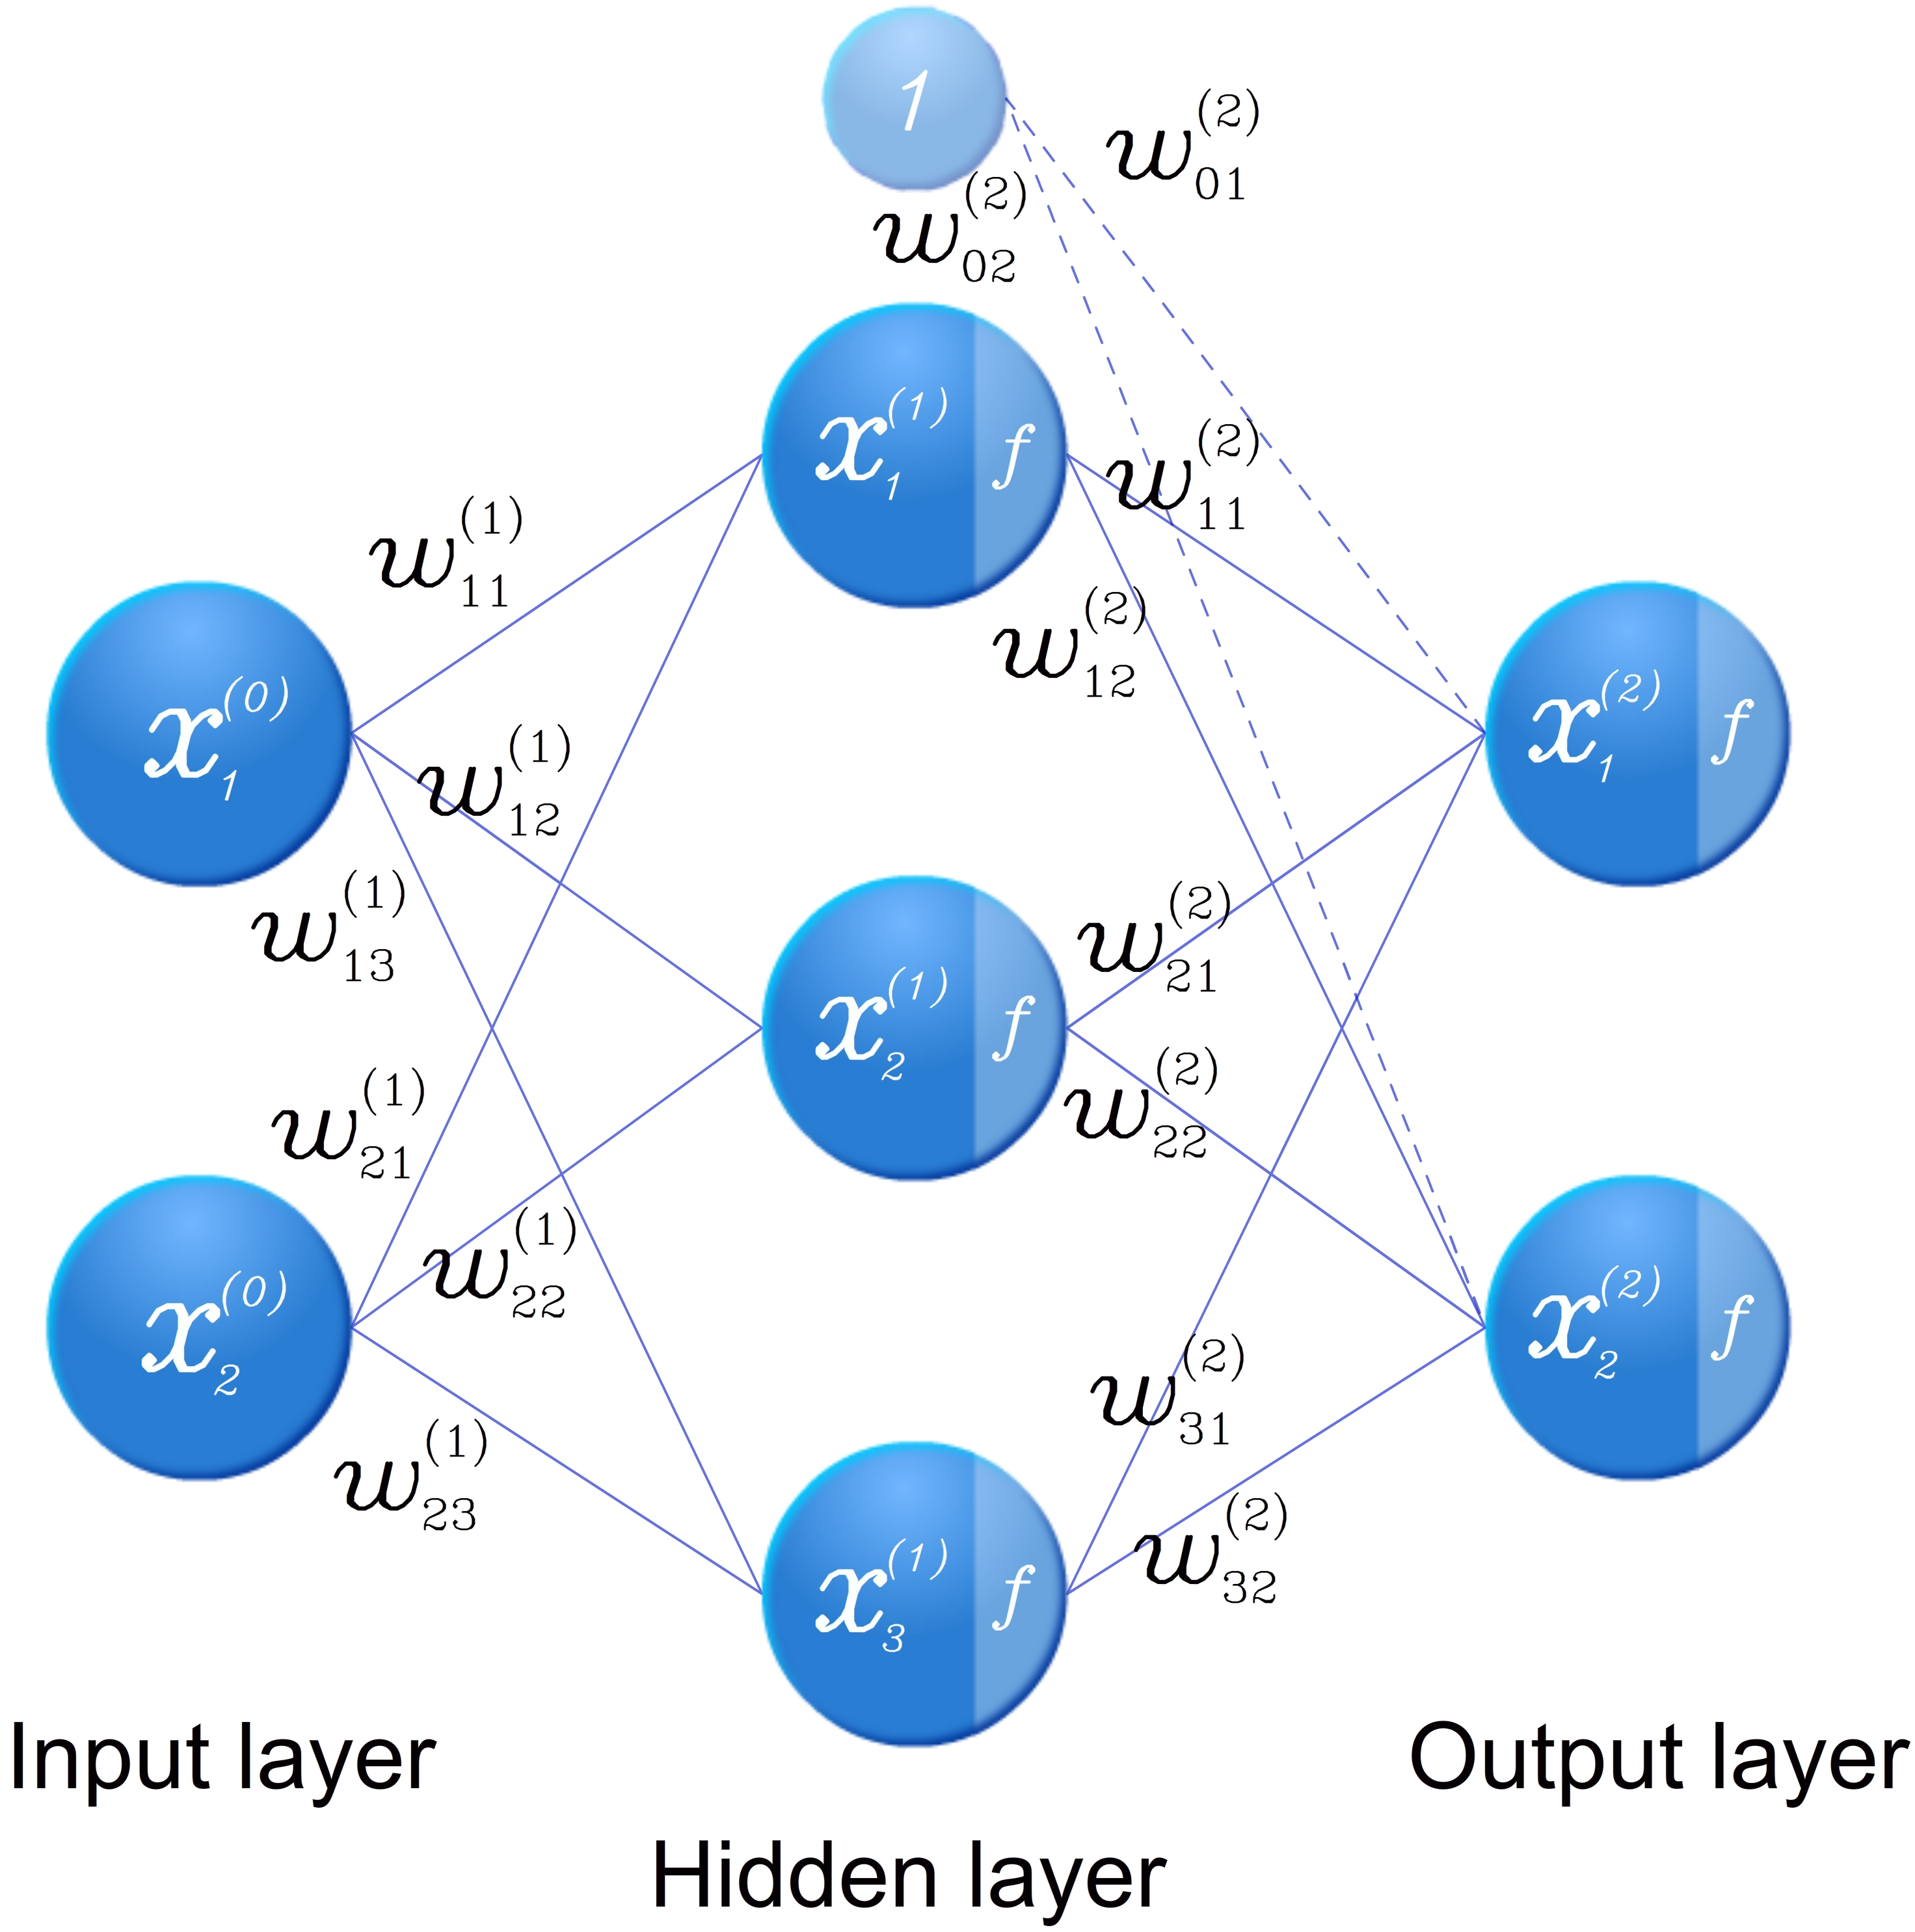
\includegraphics[scale=0.3]{figs_temp/network_graph.jpg}
	\caption{A simple neural network with 2 inputs, 2 outputs, and one hidden layer. The top node in the hidden layer is a bias term which can be added for increased flexibility during training.}
	\label{fig:ann}
\end{figure}


\subsubsection*{Hyperparameters of Neural Networks}
While some parameters, such as the sizes of the input- and output- layers, are predetermined, there are plenty of other parameters to tune in order to obtain a better model. The number of hidden layers, and nodes therein, is arbitrary, and a more complex problem may require a greater amount of these. Of course, a greater number of layers or nodes could drastically increase the number of trainable parameters, and model complexity. Another hyperparameter to consider is \textbf{bias terms}. A bias term is an external, constant input to a layer, with trainable weights assigned to it. The bias term is independent of inputs from the previous layer and increases the flexibiliy of a model, thus making it more capable of fitting to the training data \citep{kohl_2010}. The bias term is represented by the top node within the hidden layer in figure \ref{fig:ann}.

When it comes to reducing overfitting, \textbf{dropout} is a method which is commonly used together with nerual networks. By randomly selecting nodes within a layer and disabling their output, the model is forced to become more general, and does not become overfit. A node, $n$ in layer $k$ is disabled by setting the weights $w^{(k)}_{nj}$ to 0, where $j$ ranges from 1 to the number of nodes in the sequent layer. For any node in a layer that features dropout, the \textit{dropout rate} specifies the probability that the node will be disabled.

While the above parameters relate to the architecture of the network, there are additional parameters that are related to the training process. The \textbf{batch size}, for instance, specifies how many samples are propagated through the network inbetween each update of the model weights. A small batch size has the benefit of requiring little memory and converging quickly, but at the same time impairs the gradient estimate \citep{brownlee_2017}. With a larger batch size, the gradient is more accurately estimated, but the convergence is slower. 

If the total number of samples is $m$, and the batch size is $b$, there will be $\lceil \frac mb\rceil$ forward- (and backward) propagations, and equally many model weight updates. Each batch is only propagated once, but to extend the model training process even further, the number of \textbf{epochs} can be specified. This hyperparameter determines how many times each batch will be fed through the model. Often, one epoch is not enough for the weights to fully converge \citep{kriesel_2007}. However, increasing the number of epochs will definitely increase the training time, and on top of that, too many epochs puts the model at risk of becoming overfit.



\subsection*{Convolutional Neural Network + LSTM}
In previous models the data went through a feature extraction process before going into the model training. For this model, on the other hand, no feature extraction is performed. Instead, several consecutive sweeps of unprocessed IQ-data are used as input. Each range bin can be regarded as a one-dimensional time series. This motivates the use of some classification scheme that exploits temporal behaviour. Recurrent neral networks (RNNs) feature this by having feedback within individual layers in the network. \citep{karim_majumdar_darabi_chen_2018} The problem with RNNs, however, is that they suffer from a quickly vanishing gradient, and can only sustain a short term memory \citep{pascanu_mikolov_bengio_2013}. A way to combat this is to use a neural network layer type called long short term memory (LSTM).

LSTM-layers have previously been used successfully for classifications in radar applications. For instance in \citep{jithesh_sagayaraj_srinivasa_2018} the method was used in a classification model that was able to distinguish flying targets from several classes with a high accuracy. The theory behind these layers are thoroughly described in, for example \citep{hochreiter_schmidhuber_1997}

Another successful approach for time series classifications is convolutional neural networks (CNNs) \citep{karim_majumdar_darabi_chen_2018}. In \citep{capobianco_facheris_cuccoli_marinai_2017}, time series of radar data are preprocessed and used as input to a CNN. The network is used to predict what types of vehicles are driving by the radar sensor, and does so with a good success rate.


A combination of the LSTM layer and a CNN is proposed in \citep{karim_majumdar_darabi_chen_2018}. This proves to be a significant improvement from just using CCNs when classifying time series. The architecture of the model we use in this work is the same as this one, with a few tweaks of parameter values. The model essentially concatenates the outputs from a simple LSTM network and a network consiting of three one-dimensional convolution layers. For more details we refer to \citep{karim_majumdar_darabi_chen_2018}.


\section{Model evaluations}
Model evaluation is an important aspect in creating machine learning models. By using a bad evaluation strategy, one might construct a model that is seemingly good, but turns out to be useless in reality, simply because the model has been evaluated using a poorly chosen set of data. There are several things to keep in mind when testing a model's performance. One of these is to use evaluation metrics that are relevant to the type of model that is being tested. For a classification model, a common metric is accuracy, which reveals the ratio between correct predictions and total predictions. A more informative metric - at least in the case of multiclass classification - is the confusion matrix which, in addition, provides details about the model's mispredictions. Two additional metrics, suitable for classification are log-loss and AUC \citep{zheng_2015}. 

However, selecting a suitable metric is not enough. Of course, choosing what data to test your model on is equally important. By predicting on data that the model has been trained on, one could expect a very high accuracy. This accuracy, however, is not interesting at this point as a model is intended to be used on new, unseen data. For this reason, the dataset is split up in a training set and a test set in one of many ways \citep{raschka}.

One of the simplest way of dividing the dataset is to randomly select a portion of samples to use for training and use the remaining ones for evaluating the model. These two sets are commonly referred to as training- and validation sets. This can be a good way of comparing different models' performances, but it is not the ideal method for a final model evaluation. While it is true that the validation set consists of samples that the model has never seen before, it \textit{has} trained on samples close to the validation samples due to the random selection. Oftentimes closely spaced samples can have a high resemblance, and even if the model has not trained on the validation samples, it achieves a high validation accuracy because it has trained on very similar samples. Another strategy for splitting the dataset, which we will use to evaluate our models, is the leave-one-out strategy.


\subsubsection{Leave-One-Out Strategy}
The leave-one-out strategy means dividing the dataset into $n$ parts. The model evaluation is then performed in $n$ stages. For each stage, the model is trained on all data, except for one of the $n$ parts, as in figure \ref{fig:loo}. After the training, the model makes predictions of the unseen data, and the accuracy is noted. When having a small dataset - or as in this case, an arguably small amount of surfaces that have been recorded - this method is useful in that it does not require us to withhold data from the model training \citep{raschka}. It also mimics a real scenario where the model predicts on a surface it has never seen before.

In table \ref{tab:loo}, the leave-one-out results of all models above are listed for comparison.

\begin{figure}[h]
	\label{fig:loo}
	\centering
	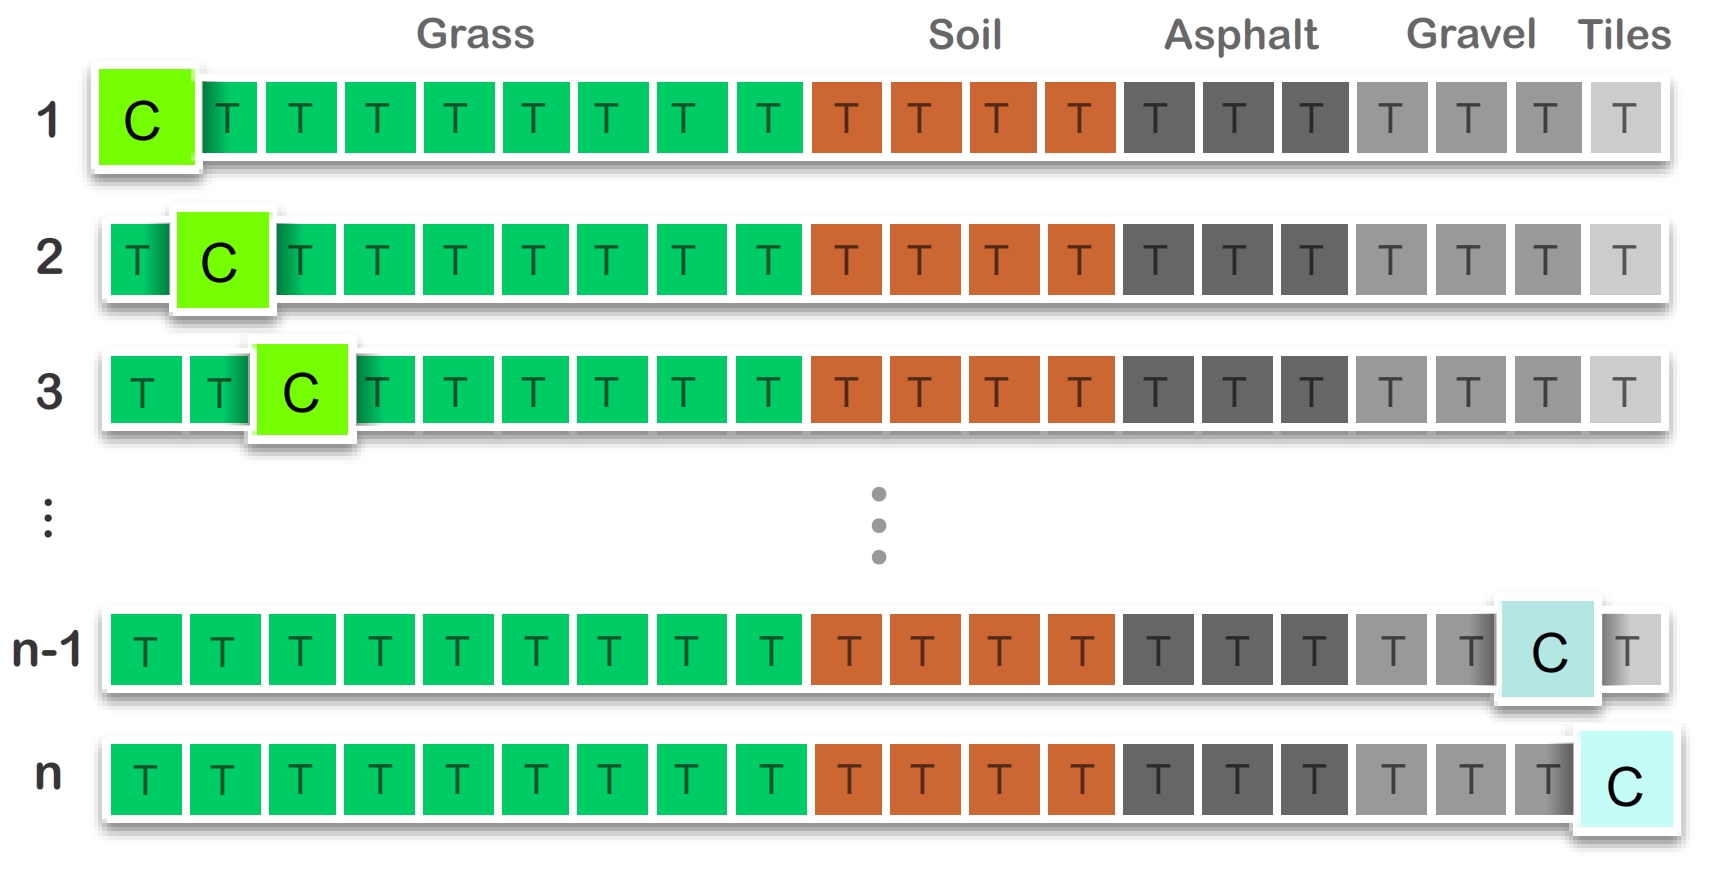
\includegraphics[scale=0.3]{figs_temp/loo.jpg}
	\caption{With the leave-one-out strategy, data is split up into $n$ parts. The model evaluation is done in $n$ steps - each time, one part of the data is excluded from the training and evaluated upon. The T's in the figure mark which parts of the data that are used for training, and the C's show what is used for classification.}
\end{figure}

%\rowcolors{2}{gray!25}{white}
\begin{table}
	\begin{center}
	\rowcolors{2}{gray!25}{white}
	\begin{adjustbox}{totalheight=\textheight-2\baselineskip}
		\begin{tabular}{|l|l|l|l|l|l|l|}
		\hline
		\rowcolor{gray!150}
		\rule{0pt}{25pt}\color{white}\textbf{Material} & \color{white}\textbf{LR} & \color{white}\textbf{RF} & \color{white}\textbf{\shortstack{LSTM\\CNN}} & \color{white}\textbf{SVM} & \color{white}\textbf{LDA} & \color{white}\textbf{DNN}\\
		Grass 1 & 97.9 & 98.05 & \cellcolor{red!20}59.0 & 95.75 & 96.8 & 97.45\\
		Grass 2 & 99.8 & 99.5 & \cellcolor{red!20}83.8 & 96.2 & 100.0 & 99.95\\
		Grass 3 & 94.35 & \cellcolor{red!20}86.75 & 94.5 & 91.4 & 92.6 & 95.3\\
		Grass 4 & 95.7 & 96.45 & 100.0 & 91.35 & 93.65 & 97.8\\
		Grass 5 & 96.65 & 97.25 & 97.4 & 93.95 & 95.9 & 95.55\\
		Grass 6 & 96.35 & 98.8 & 95.9 & 92.95 & 97.2 & 99.3\\
		Grass 7 & 99.9 & 99.85 & 99.9 & 99.65 & 99.95 & 100.0\\
		Grass 8 & 97.0 & 96.65 & 97.5 & 96.85 & 92.7 & 96.95\\
		Grass 9 & 97.75 & 97.7 & 99.8 & 97.8 & 96.3 & 98.75\\
		Grass 10 & 99.2 & 98.65 & 99.9 & 99.0 & 97.65 & 99.7\\
		Grass 11 & 99.35 & 98.7 & 99.9 & 99.25 & 97.55 & 99.8\\
		Grass 12 & 99.6 & 99.4 & 99.9 & 99.6 & 99.2 & 99.65\\
		Grass 13 & 100.0 & 100.0 & 100.0 & 100.0 & 99.85 & 100.0\\
		Grass 14 & 96.35 & 96.8 & 98.6 & 95.6 & \cellcolor{red!20}89.85 & 98.1\\
		Grass 15 & 97.6 & 95.45 & 99.8 & 93.1 & \cellcolor{red!20}87.4 & 99.05\\
		Grass 16 & 97.55 & 98.0 & 99.8 & 95.8 & 94.05 & 98.85\\
		Grass 17 & 95.4 & 92.85 & 98.4 & 94.6 & \cellcolor{red!20}89.9 & 95.0\\
		Grass 18 & 97.35 & 94.4 & 96.9 & 96.55 & 93.65 & 95.6\\
		\hline
		Asphalt 1 & 100.0 & 100.0 & 99.9 & 100.0 & 100.0 & 100.0\\
		Asphalt 2 & 99.95 & 100.0 & 99.0 & 100.0 & 100.0 & 100.0\\
		Asphalt 3 & 100.0 & 100.0 & 99.7 & 100.0 & 99.95 & 99.2\\
		Asphalt 4 & 99.9 & 99.85 & 100.0 & 99.9 & 99.95 & 100.0\\
		Asphalt 5 & 100.0 & 100.0 & 100.0 & 100.0 & 100.0 & 100.0\\
		Asphalt 6 & 100.0 & 100.0 & 100.0 & 100.0 & 99.9 & 99.95\\
		\hline
		Gravel 1 & 99.45 & 99.85 & 99.8 & 99.9 & 99.2 & 99.7\\
		Gravel 2 & \cellcolor{red!20}82.65 & 97.1 & \cellcolor{red!20}86.6 & \cellcolor{red!20}88.2 & \cellcolor{red!20}89.3 & 94.3\\
		Gravel 3 & 99.95 & 99.55 & 100.0 & 100.0 & 99.95 & 99.75\\
		Gravel 4 & 98.95 & 99.6 & 99.9 & 99.55 & 99.9 & 99.8\\
		Gravel 5 & 99.85 & 99.8 & 99.9 & 99.95 & 100.0 & 99.7\\
		Gravel 6 & 99.75 & 99.7 & 100.0 & 99.75 & 99.9 & 99.55\\
		\hline
		Soil 1 & 99.85 & 100.0 & 99.7 & 99.95 & 99.7 & 99.9\\
		Soil 2& 99.35 & 99.6 & 99.4 & 99.85 & 99.4 & 99.75\\
		Soil 3 & 99.75 & 99.85 & 100.0 & 100.0 & 99.9 & 99.85\\
		Soil 4 & 97.8 & 96.3 & \cellcolor{red!20}88.9 & 98.9 & 97.4 & 95.95\\
		Soil 5 & 96.25 & 95.45 & 100.0 & 96.55 & 96.55 & 93.95\\
		Soil 6 & 96.35 & 94.0 & 99.3 & 96.85 & 95.5 & 99.85\\
		Soil 7 & 92.65 & 95.15 & 99.3 & 90.25 & 92.4 & 100.0\\
		Soil 8 & 94.75 & 95.65 & \cellcolor{red!20}84.7 & 90.95 & 92.9 & 95.15\\
		\hline
		Tiles 1 & 99.35 & 99.4 & 100.0 & 99.55 & 99.3 & 99.35\\
		Tiles 2 & 99.95 & 99.75 & 99.9 & 99.95 & 99.6 & 99.95\\
		Tiles 3 & 99.95 & 99.9 & 100.0 & 100.0 & 100.0 & 99.95\\
		Tiles 4 & 99.95 & 99.7 & 99.5 & 99.95 & 100.0 & 94.45\\
		\hline
		\textbf{Mean} & 97.96 & 97.99 & 97.06 & 97.37 & 97.02 & \cellcolor{green!20}98.5\\
		\textbf{Median} & 99.35 & 99.4 & \cellcolor{green!20}99.8 & 99.4 & 99.2 & 99.68\\
		\textbf{SD} & 3.05 & 2.63 & 7.23 & 3.3 & 3.58 & \cellcolor{green!20}1.96\\
		\hline
		\end{tabular}
	\end{adjustbox}
	\end{center}
	\caption{Leave-one-out accuracies for all collected data series and the different models.}
	\label{tab:loo}
\end{table}

\subsubsection{Selecting a Model}
Optimizing each model presented above would of course be ideal, but also require much time and effort. Hence, we select what we regard as the most promising model based on the result of the leave-one-out evaluation. This model will then be optimized and more thoroughly evaluated.

Table \ref{tab:loo} shows the leave-one-out results for all models. From the table we can see that all models perform well on every asphalt- and tiled surfaces. Gravel-, soil- and grass-surfaces, however, can sometimes be harder to classify for the models. Looking back at the principal component analysis in figure 4.4, this is what we could have expected due to the wide spread, and slight overlap between the samples within these categories. As for gravel, there is one measurement in particular that sticks out - gravel 2. The accuracy of this is well below the average accuracy for all models. This could be that this particular gravel contains characteristics which are not captured by the other non-grass surfaces, resulting in several misclassifications. It could also be that some temporary problem occured while measuring, for example that the radar jumped out of its socket.

Another quirk worth noting is the great accuracy span of the LSTM- \& CNN method. While it has a leading median score of 99.8 \%, it also contains several dips to some of the lowest accuracies of all models. This gives it a high standard deviation compared to the other models, suggesting it is less robust. It is possible that this could be remedied with a little bit of fine-tuning, but due to a limited amount of time, we disregard the LSTM-model, and the DNN-model becomes the one with the greatest median and mean as well as the lowest standard deviation. 

After optimizing the hyperparameters of the DNN, using \textit{Hyperas}, the network in figure \ref{fig:opt_net} is obtained. The two hidden layers have 24 and 12 nodes and dropout rates of 14 and 2 percent, respectively. Both layers have an activation function, $f(x)=\textrm{max}(0,x)$, often referred to as rectified linear unit (ReLU) and the output layer has a \textit{softmax} activation function. Furthermore the batch size in the learning phase is 32, and the number of epochs is set to 20. Finally, the optimization algorithm prefered by Hyperas is RMSprop.

\begin{figure}[h]
	\centering
	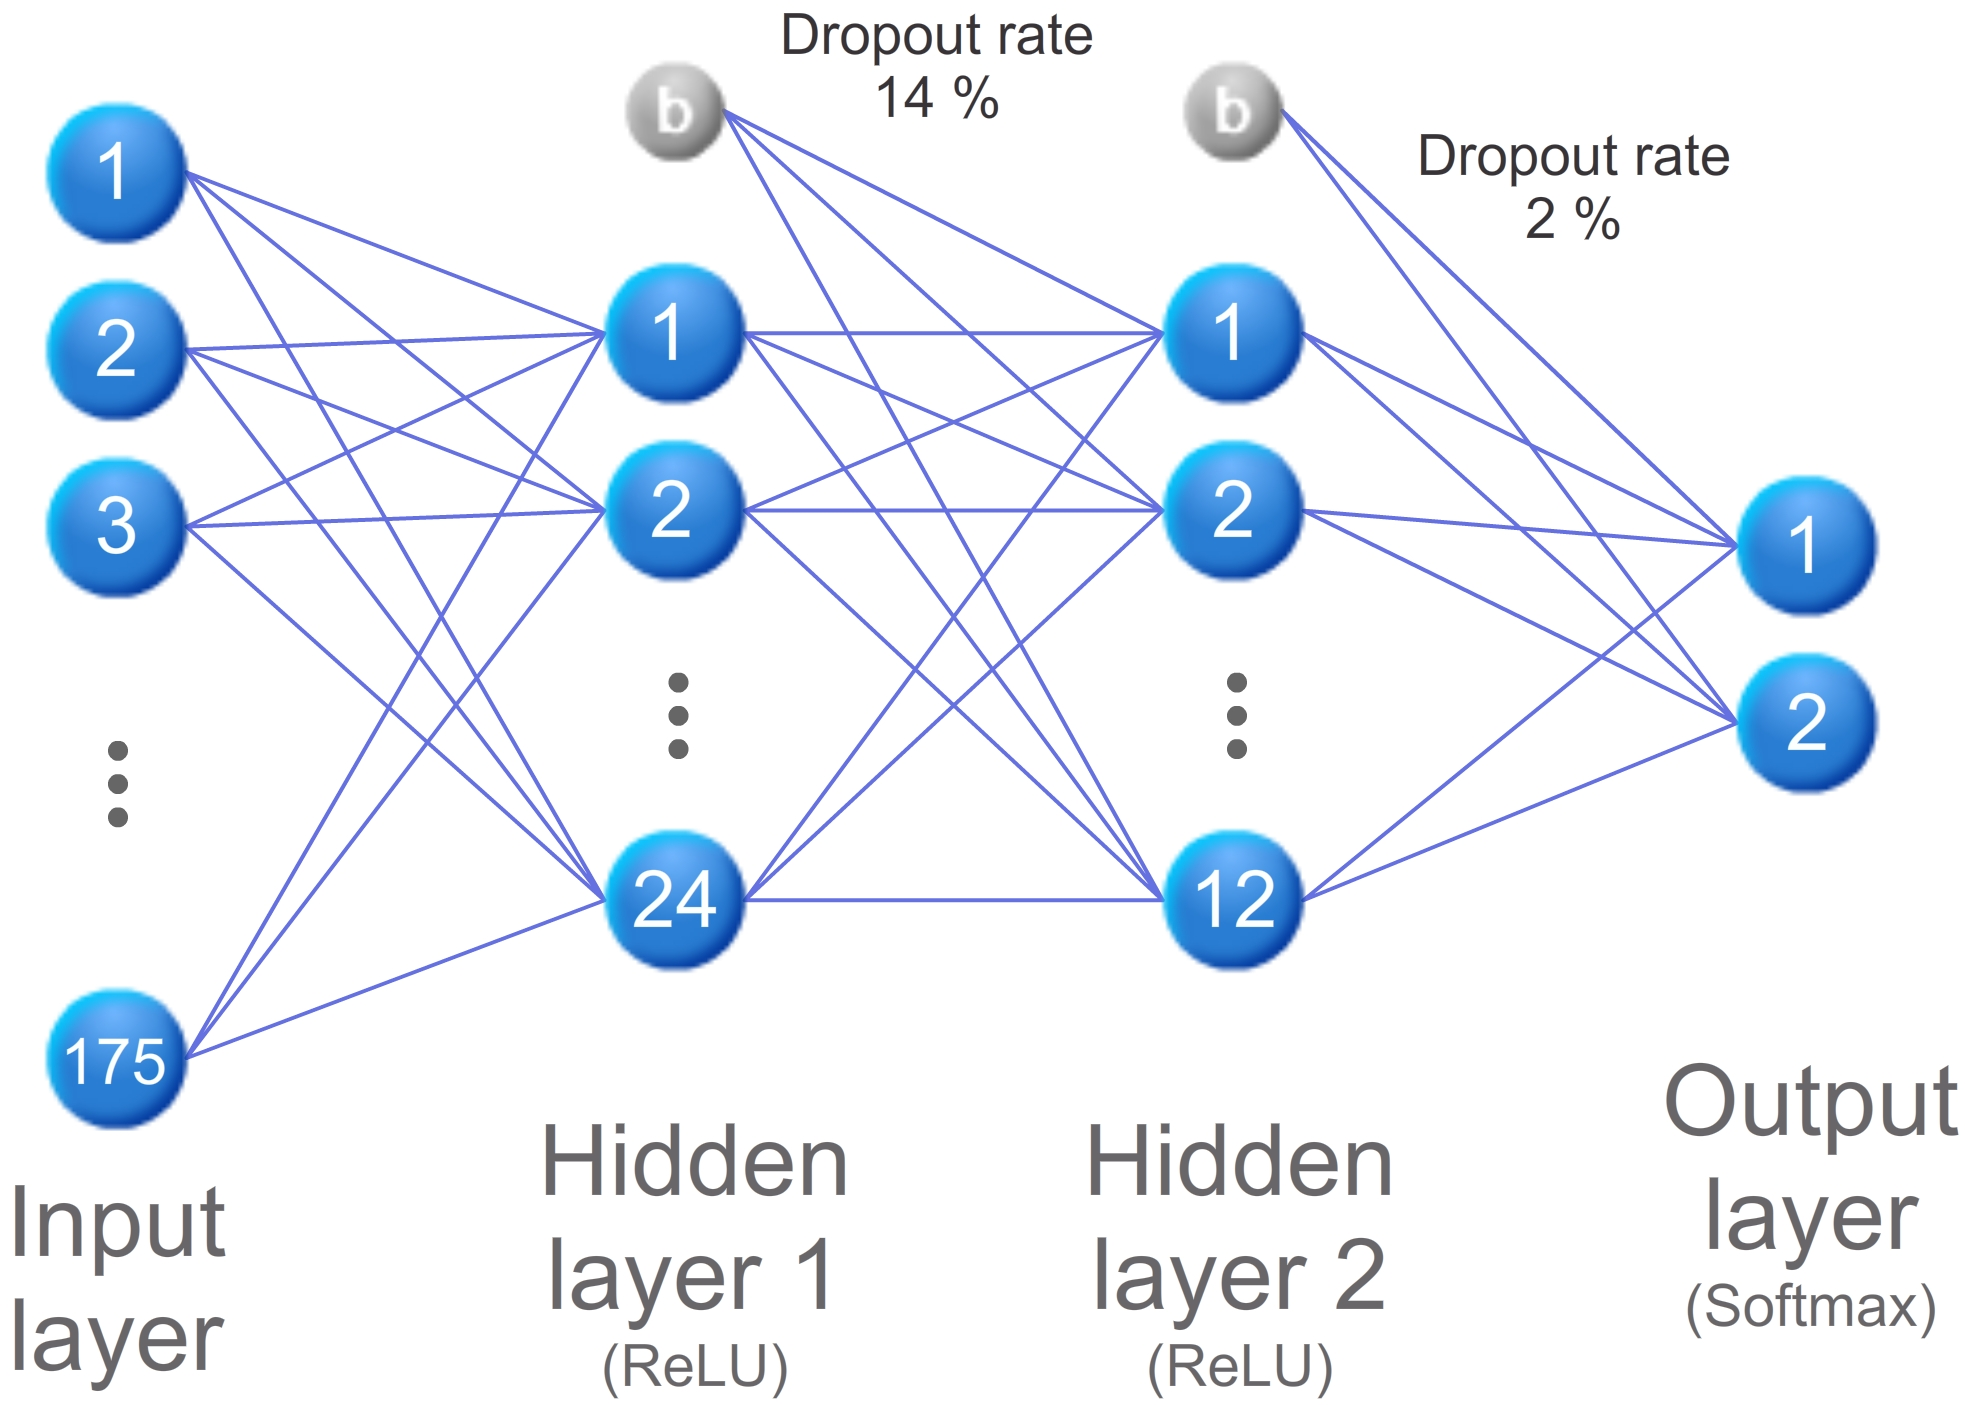
\includegraphics[scale=0.5]{figs_temp/optimized_network_graph.jpg}
	\caption{Using Hyperas, a network with two hidden layers was optimized in terms of number of nodes, dropout rate and activation function among other things. The resulting network has 24 and 12 nodes in the hidden layers, and dropout rates of 14 and 2 percent, respectively. The hidden layers were assigned the ReLU activation function.}
	\label{fig:opt_net}
\end{figure}








